This laboratory focused on practical implementations of serial-bus communication using the I\textsuperscript{2}C protocol, interfacing external devices through the STM32's HAL (Hardware Abstraction Layer). 
The aim was to interface a Pololu QTR reflectance line sensor and a 16-key matrix keypad using two SX1509 I/O expanders connected to the STM32F767 microcontroller through a shared I\textsuperscript{2}C bus. 
The activity covered embedded systems concepts, including interrupt handling, keypad scanning, sensor polling, and dynamic control of an LED.

\subsection{Theoretical background}



% PROBLEM ANALYSIS
% Interfacing multiple I\textsuperscript{2}C slave devices on a shared bus requires managing device addresses, selecting the correct internal registers, and interpreting device-specific data. For real-time responsiveness - such as reacting to a key press - external interrupts are used instead of continuous polling. This lab combined both techniques: polling was used for the line sensor, while interrupts were used for detecting keypad input. 


%Additionally, implementing responsive user interaction through interrupts and traslating raw binary data into usable application logic.

%%%%%%%%%%%%%%%%%%%%%%%%%

\subsubsection{I\textsuperscript{2}C \& HAL Interface}

The Inter-Integrated Circuit (I\textsuperscript{2}C) is a syncronous, multi-master, multi-slave serial communication protocol widely used in embedded systems for short-distance communication. 
It is especially useful when multiple devices share the same bus, as in the case of this laboratory. 
I\textsuperscript{2}C uses two bidirectional lines:

\begin{itemize}
    \item \textbf{SCL} (Serial Clock Line): carries the clock signal generated by the master
    \item \textbf{SDA} (Serial Data Line): transmits and receives data between master and slaves.
\end{itemize}

\noindent
Each I\textsuperscript{2}C communication involves the master initiating a transmission, specifying an address to select a slave device, followed by a read or write operation to specific registers on that device. 
\noindent
To simplify I\textsuperscript{2}C communication, the STM32 HAL (Hardware Abstraction Layer) provides high-level functions that handle the complex low-level protocol mechanics (e.g. generating START/STOP condition, clock stretching and byte-level ACK/NACKs). The two most important functions used in this lab are:


\begin{itemize}
    \item \texttt{HAL\_StatusTypeDef HAL\_I2C\_Mem\_Read()} - to read data from a slave register
    \item \texttt{HAL\_StatusTypeDef HAL\_I2C\_Mem\_Write()} - to write data to a slave register
\end{itemize}

This mechanism was used throughout the lab for example to read the current keypad status and to acquire sensor data from the QTR sensor.


\subsubsection{External Interrupts on STM32}

An interrupt is a hardware-triggered mechanism that suspends the main execution flow, allowing immediate response to input (e.g., key press). In embedded systems, external interrupts are critical for handling asynchronous inputs without polling, improving efficiency and responsiveness. 

STM32 microcontrollers use the EXTI (External Interrupt) peripheral to detect changes on GPIO pins and generate interrupts accordingly. To set up an external interrupts, the target GPIO pin is configured as an input with interrupt capability and the desired trigger edge (rising, falling, or both) is selected. The pin is then mapped to the appropriate EXTI line, the interrupt is unmasked and enabled in the NVIC with a set priority. Once configured, a signal edge on the pin triggers an interrupt that temporarily halts normal execution. STM32'S HAL processes this interrupt through a centralized interrupt service routine (ISR), which subsequently invokes a user-defined callback function: 

\begin{itemize}
    \item \texttt{HAL\_GPIO\_EXTI\_Callback(uint16\_t GPIO\_Pin)}, responsible for handling the interrupt and enabkling the application
\end{itemize}






In this laboratory, an external interrupt was configured on PF4, triggered by SX1509\_2 when a key was pressed on the keypad.


\subsection{System Configuration}
\label{sec:system_configuration}

\begin{itemize}
    \item \textbf{Microcontroller:} STM32F767
    \item \textbf{I\textsuperscript{2}C Bus:}: shared on I2C1
    \begin{itemize}
        \item \textbf{SX1509\_1} (address \texttt{0x3E}): interfaces line sensor interface.
        \item \textbf{SX1509\_2} (address \texttt{0x3F}): serves as the keypad controller.
    \end{itemize}
    \item \textbf{Interrupts:}: the NINT output of SX1509\_2 is connected to PF4 on the microcontroller and configured as GPIO\_EXTI4. This interrupt is triggered on a falling edge when a keypad button is pressed.
    \item \textbf{LED:} connected to PE5, used as output indicator.
\end{itemize}

This laboratory includes structured testing of HAL I\textsuperscript{2}C communication functions and SX1509 registers as detailed in Sections 2.4-2.6 of the handout.

\bigskip


%Two sx1509 are used to interact with the line sensor (Pololu QTR Reflectance Sensor) and with a 16-key keypad. These two devices are connected to the microcontroller through the I2C bus \((\mathbf{I2C\_1})\) and share the same i2c line. Each of them is associated to a different slave address, the first called \( SX1509_1\) is assigned to 0x3E (LINE SENSOR), while the second one \( SX1509_1\) is assigned to address 0x3F (KEYPAD).

%The keypad device is capable of rising an interrupt through the pin NINT which is connected with the pin PF4 (GPIO\_EXTI4\_KPAD\_IR) of the microcontroller STM32F7. 


\begin{figure}[H]
    \centering
    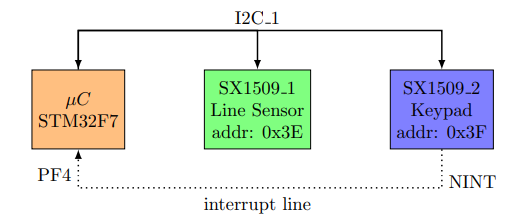
\includegraphics[width=0.55\linewidth]{lab1-2/figures/I2C_scheme.png}
    \caption{I\textsuperscript{2}C connection scheme}
    \label{fig:I2C}
\end{figure}


\subsubsection{Procedure}

In the laboratory setup, to enable the interrupt on pin PF4, the \texttt{*.ioc} configuration file was modified by setting PF4 to \texttt{GPIO\_EXTI4} (GPIO\_EXTI4\_KPAD\_IR). The interrupt trigger mode was configured in \emph{External Interrupt Mode with Falling edge trigger detection}, and the pull-up/pull-down resistors were disabled by selecting \emph{No pull-up and no pull-down}. Additionally, to enable the \texttt{printf} function for debugging purposes, the Serial Wire Viewer (SWV) was activated. 

\subsubsection{SX1509 Register Map}

The SX1509 data registers employed in this lab include: 

\begin{itemize}
    \item \texttt{0x10}: \texttt{REG\_DATA\_B} contains the data of the line sensor
    \item \texttt{0x27}: \texttt{REG\_KEY\_DATA\_1} contains the  status of the column of the keypad (8-bit values)
    \item \texttt{0x28}: \texttt{REG\_KEY\_DATA\_2} contains the  status of the row of the keypad (8-bit values)
\end{itemize}

\subsubsection{Keypad}

A 4x4 matrix keypad is interfaced with the microcontroller through the SX1509\_2 I/O expander, which communicates via the I\textsuperscript{2}C. The Keypad is structured as a matrix composed of 4 rows and 4 columns, resulting in 16 unique keys. Each key press electrically connects a specific row to a specific column, enabling the identification of the key based on its position in the matrix. 

To detect key presses, the SX1509 uses an internal scanning engine. The columns are configured as open drain outputs, while the rows are configured as input with internal pull-up resistors. When a key is pressed, it creates a path to ground between the active column and the corresponding row, causing the associated row input to be pulled low. The idle state (no key pressed), all bits are high (logic '1'), i.e., the register values are 0xFF (255 in decimal). When a  key is pressed, the corresponding bits in both registers are pulled low (logic '0'). Each bit in the register corresponds to a specific row or column, with bit 0 (Least Significant Bit, LSB) representing the first row or column, and subsequent bit representing lines in order. \\

\begin{figure}[H]
    \centering
    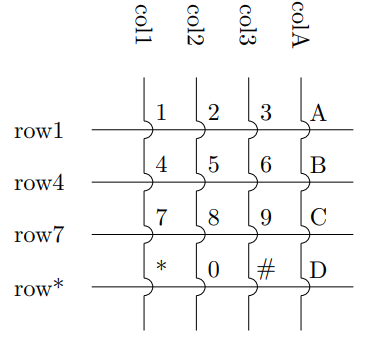
\includegraphics[width=0.45\linewidth]{lab1-2/figures/keypad.png}
    \caption{Keypad scheme}
    \label{fig:keypad}
\end{figure}

\noindent
For example, if the key '8' is pressed (located at row 3, column 2), the SX1509 will return: 

\begin{itemize}
    \item \texttt{REG\_KEY\_DATA\_1} $ =0xFD=0b11111101$ $\rightarrow$ bit 1 (column 2) is low 
    \item \texttt{REG\_KEY\_DATA\_2} $=0XFB=0b11111011$ $\rightarrow$ bit 2 (row 3) is low 
\end{itemize}

\noindent
This binary information allows the software to determine the pressed key by evaluating the position of the zero bits. The microcontroller responds to this event by handling an interrupt (generated on the NINT pin connected to PF4), and reading these two registers using the HAL I\textsuperscript{2}C function \texttt{HAL\_I2C\_Mem\_Read(\&hi2c1, SX1509\_I2C\_ADDR2 << 1, REG\_KEY\_DATA\_1, 1, \&col, 1, I2C\_TIMEOUT)}. The row and column indices are then mapped to a specific character using a predefined lookup table that corresponds to the keypad layout. 

\noindent
This method provides an efficient and reliable way to detect and decode user input from a matrix keypad in embedded systems applications.

%The Keypad is a 4x4 matrix, where each row and column are connected to a set GPIO pins of the device SX1509\_2 using a pull-up resistor. As mentioned above, the status of the key is stored in the registers..
%The least significant bit of the reg1 correspond to the column 1, the second to the column 2 and so on. The same applies to the reg2 ...
%Explain how to understand which key has been pressed...

\subsubsection{Line Sensor (Pololu QTR Reflectance)}
\label{sec:line_sensor}

\noindent
The Pololu QTR reflectance sensor array is a digital infrared sensing system design to detect reflectivity, utilized in Laboratory 4 for line-following applications. It comprises multiple emitter-phototransistor pairs that measure the intensity of reflected infrared light to distinguish between reflective (e.g. white) and non-reflective (e.g. black) surfaces.
In this laboratory setup, the QTR sensor interfaces with the STM32 microcontroller through an SX1509 I/O expander(I2C addres: 0X3E), enabling communication over a shared I\textsuperscript{2}C bus. 
Each sensor in the array operates by charging a capacitor through its phototransistor and then measuring the capacitor's discharge time. On reflective surfaces, the phototransistor saturates, causing rapid discharge and resulting in a short high-pulse duration, interpreted as a logical '1'. Conversely, dark surfaces reflect less infrared light, resulting in slower discharge and longer high pulse, which is thresholded as a logical '0'. This binary abstraction enables digital readout of surface reflectivity:

\begin{itemize}
    \item High (logic 1): White or reflective surface.
    \item Low (logic 0): Black surface.
\end{itemize}


\noindent
The digital outputs of the sensor array are connected to the SX1509's input pins and read the digital state of each sensor line through its register \texttt{REG\_DATA\_B} (address 0x10). The STM32 polls this register using the following HAL function: \\
\texttt{HAL\_I2C\_Mem\_Read(\&hi2c1, SX1509\_I2C\_ADDR1 <<1, REG\_DATA\_B, 1, \&sensor\_line, 1, I2C\_TIMEOUT)}. \\
Each bit in the texttt{sensor\_line} variable corresponds to the the state of an individual sensor element, encoding the presence and relative position of a detected line. This discrete, low-latency data stream provides reliable surface detection, forming the basis for the real-time line-following algorithm implemented in Laboratory 4.


\subsubsection{LED}

The LED used in this experience is connected to pin PE5 (Port E, Pin 5) on the STM32 microcontroller. The LED is directly interfaced with the GPIO through a current limiting resistor (R1), which protects the LED by controlling the current flow. 
The LED is controlled using STM32'S HAL functions. The most relevant function for setting the LED state is: 

\begin{itemize}
    \item \texttt{HAL\_GPIO\_WritePin(GPIOE, GPIO\_PIN\_5, GPIO\_PIN\_SET)}
    \item \texttt{HAL\_GPIO\_ReadPin(GPIOE, GPIO\_PIN\_5)}
    \item \texttt{HAL\_GPIO\_TogglePin(GPIOE, GPIO\_PIN\_5)}
\end{itemize}

This setup allows the LED to be used as a visual indicator in response to GPIO interrupts.


%\subsection{Setup \& Initialization}


\subsection{Code implementation}

--- HAL function - also HAL\_GPIO\_EXTI\_Callback()
    

\subsubsection{Exercise 1 - Keypad interrupt and register read}

An external interrupt callback \texttt{HAL\_GPIO\_EXTI\_Callback()} handles the interrupt from the SX1509 keypad engine on key press (NINT signal). 
The ISR must:

\begin{itemize}
    \item Identify the EXTI pin triggering the event.
    \item Use \texttt{HAL\_I2C\_Mem\_Read()} to read key status registers \texttt{REG\_KEY\_DATA\_1} and \texttt{REG\_KEY\_DATA\_2}.
    \item Print the interrupt source with \texttt{printf()} for debugging feedback.
\end{itemize}

\bigskip

\begin{lstlisting}[language=C]
void HAL_GPIO_EXTI_Callback(uint16_t GPIO_Pin)
{
   // EXERCISE 1

   printf("Interrupt on pin (%d).\n", GPIO_Pin);

   uint8_t col;
   uint8_t row;
   HAL_StatusTypeDef status_col = HAL_I2C_Mem_Read(&hi2c1, SX1509_I2C_ADDR2 << 1, 
   REG_KEY_DATA_1, 1, &col, 1, I2C_TIMEOUT); //col
   HAL_StatusTypeDef status_row = HAL_I2C_Mem_Read(&hi2c1, SX1509_I2C_ADDR2 << 1, 
   REG_KEY_DATA_2, 1, &row, 1, I2C_TIMEOUT); //row

   printf("col = %d\n", col);
   printf("row = %d\n", row);

   ...

}
\end{lstlisting}

\subsubsection{Exercise 2 - Key decoding and display}

In this exercise, we have detect which key was pressed using the cleared bit in column and row readings and then map it using the keypad layout array.

\bigskip

\begin{lstlisting}[language=C]
const char keypadLayout[4][4] = {
    {'*', '0', '#', 'D'},
    {'7', '8', '9', 'C'},
    {'4', '5', '6', 'B'},
    {'1', '2', '3', 'A'}};

void HAL_GPIO_EXTI_Callback(uint16_t GPIO_Pin)
{
   ...
   // EXERCISE 2

   int row_index = -1, col_index = -1;

   // Ogni bit basso (0) rappresenta il tasto premuto
   // 0b11111110 = 254 -bit 0 e' 0, quindi indice 0
   // 0b11111101 = 253 -> bit 1 e' 0, quindi indice 1
   // 0b11111011 = 251 -> bit 2 e' 0, quindi indice 2
   // 0b11110111 = 247 -> bit 3 e' 0, quindi indice 3

   switch (row) {
     case 254: row_index = 0; break;
     case 253: row_index = 1; break;
     case 251: row_index = 2; break;
     case 247: row_index = 3; break;
   }

   switch (col) {
     case 254: col_index = 0; break;
     case 253: col_index = 1; break;
     case 251: col_index = 2; break;
     case 247: col_index = 3; break;
   }

   if (row_index != -1 && col_index != -1) {
     button = keypadLayout[row_index][col_index];
     printf("button = %c \n", button);
   } else {
     printf("Invalid key press: col = %d, row = %d\n", col, row);
   }
   
   ...

}

\end{lstlisting}


\begin{figure}[H]
    \centering
    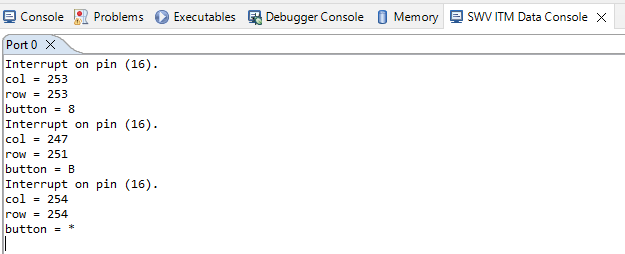
\includegraphics[width=0.75\linewidth]{lab1-2/figures/exercise3.1-3.2.PNG}
    \caption{Printf of the exercise 1-2}
    \label{fig:ex3.2}
\end{figure}


%%%%%%%%%%
%%%%%%%%%%
%%%%%%%%%%
DA RIVEDERE FUNZIONAMENTO KEYPAD
%%%%%%%%%%
%%%%%%%%%%

\subsubsection{Exercise 3 - Line Sensor polling}

In this exercise we need to read the line sensor's state and for doing this we have read the register \texttt{REG\_DATA\_B} using the HAL function \texttt{HAL\_I2C\_Mem\_Read()}. Then we introduce a poll line sensor every 100 ms using \texttt{HAL\_Delay}.

\bigskip

\begin{lstlisting}[language=C]
while (1)
{
    /* USER CODE END WHILE */
    /* USER CODE BEGIN 3 */
    // EXERCISE 3
    
    uint8_t sensor_line;
    HAL_StatusTypeDef status_sens_line = HAL_I2C_Mem_Read(&hi2c1, 
    SX1509_I2C_ADDR1 << 1, REG_DATA_B, 1, &sensor_line, 1, I2C_TIMEOUT);
    printf("status sensor line %d\n", sensor_line);
    HAL_Delay(100);

}

\end{lstlisting}

\subsubsection{Exercise 4 - LED Blinking with dynamic frequency}


(SIMPLE WAY)
\noindent
The key press is captured via the keypad interrupt in \texttt{HAL\_GPIO\_EXTI\_Callback()} and the LED blinking is handled in the while(1) loop.

\bigskip

\noindent
\begin{lstlisting}[language=C]

while (1)
{
    /* USER CODE END WHILE */

    /* USER CODE BEGIN 3 */
   // EXERCIZE 4.1
   if(button < '1' || button > '9'){
     button = '0';
     HAL_GPIO_WritePin(GPIOE, GPIO_PIN_5, GPIO_PIN_RESET);
     continue;
   }
   uint8_t freq = (uint8_t)button - '0';
   HAL_GPIO_TogglePin(GPIOE, GPIO_PIN_5);
   period = 1000/freq;
   HAL_Delay(period/2);

}


\end{lstlisting}


\bigskip
\noindent
(HARD WAY)
We have used the Keypad input to set LED blink frequency. Upon $\#$, the collected digits are converted to an integer. 

%Correct keypress stored in input_buffer[], max three digits. #triggers conversion to integer: target_freq = atoi(input_buffer);
%invalid keys reset the buffer

\bigskip
\noindent
\begin{lstlisting}[language=C]

void HAL_GPIO_EXTI_Callback(uint16_t GPIO_Pin)
{
   ...
   // EXERCISE 4.2

   if (row_index != -1 && col_index != -1) {
     button = keypadLayout[row_index][col_index];
     printf("button = %c \n", button);
     if (button >= '0' && button <= '9') {
       if (input_index < 3) {
         input_buffer[input_index++] = button;
       }
     } else if (button == '#') {
       input_buffer[input_index] = '\0'; // chiusura stringa
       target_freq = atoi((char*)input_buffer); // converte la stringa in intero
       freq_ready = 1;
       input_index = 0; // reset buffer
     } else if (button < '0' || button > '9') {
       // reset se tasto errato o A/B/C/D/*
       input_index = 0;
       target_freq = 0;
       memset((char*)input_buffer, 0, sizeof(input_buffer));
     }
   } else {
     printf("Invalid key press: col = %d, row = %d\n", col, row);
   }

}

\end{lstlisting}

\begin{lstlisting}[language=C]
while (1)
{
   /* USER CODE END WHILE */

    /* USER CODE BEGIN 3 */
   // EXERCISE 4.2

   if (freq_ready && target_freq > 0) {
     uint32_t period = 1000 / target_freq; // periodo in ms
     HAL_GPIO_TogglePin(GPIOE, GPIO_PIN_5);
     HAL_Delay(period / 2); // meta' on, meta' off
   } else {
     HAL_GPIO_WritePin(GPIOE, GPIO_PIN_5, GPIO_PIN_RESET);
     HAL_Delay(100); // idle
   }

}


\end{lstlisting}

\subsection{Results}




\subsection{Conclusion}

This laboratory successfully demonstrated I\textsuperscript{2}C device integration using STM32 HAL, including multi-device communication, external interrupts, register-level control and real-time response to user input. 
